% 2020 江苏卷 22：三棱锥 A-BCD，O 为 BD 中点，E 为 AC 中点，F 在 BC 上（BF=BC/4）
% 绘制依据：固定源 PDF 第 1116 面原图。A 在上，B 左下，C 右，D 在内部（被遮挡），
% 可见棱 AB、AC（含 AE、EC）、BC（含 BF、FC）与面 ABC 内的 EF 为实线；
% 隐蔽棱 AD、AO、BD（含 BO、OD）、DC、DE 为虚线。标出 A、B、C、D、O、E、F。
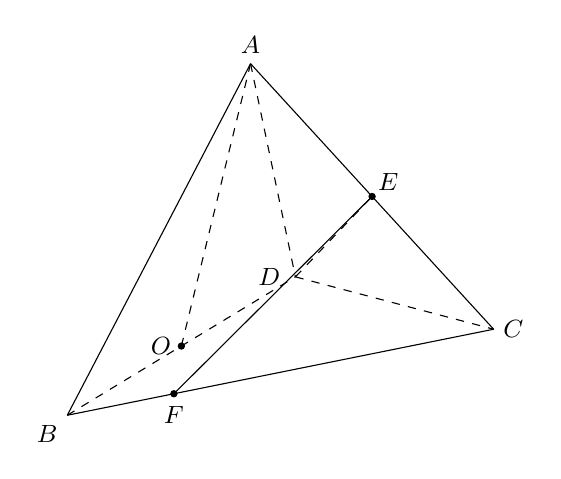
\begin{tikzpicture}[scale=0.95, font=\small]
  \coordinate (A) at (2.45,4.70);
  \coordinate (B) at (0.00,0.00);
  \coordinate (C) at (5.70,1.15);
  \coordinate (D) at (3.05,1.85);
  \coordinate (O) at (1.525,0.925);
  \coordinate (E) at (4.075,2.925);
  \coordinate (F) at (1.425,0.2875);

  % 可见棱
  \draw (A) -- (B);
  \draw (A) -- (E) -- (C);
  \draw (B) -- (F) -- (C);
  \draw (E) -- (F);
  % 隐蔽棱
  \draw[dashed] (A) -- (D);
  \draw[dashed] (A) -- (O);
  \draw[dashed] (B) -- (D);
  \draw[dashed] (D) -- (C);
  \draw[dashed] (D) -- (E);

  \fill (O) circle (1.4pt);
  \fill (E) circle (1.4pt);
  \fill (F) circle (1.4pt);
  \node[above] at (A) {$A$};
  \node[below left] at (B) {$B$};
  \node[right] at (C) {$C$};
  \node[left=2pt] at (D) {$D$};
  \node[left=1pt, inner sep=2.5pt] at (O) {$O$};
  \node[above right, inner sep=2pt] at (E) {$E$};
  \node[below=2pt, inner sep=2.5pt] at (F) {$F$};
\end{tikzpicture}
